\documentclass{article}
\usepackage[a4paper, portrait, margin=1in]{geometry}
\usepackage{tabularx}
\usepackage{graphicx}
\usepackage{amsmath}
\usepackage{amsfonts}
\usepackage{algorithm}
\usepackage[noend]{algpseudocode}


\title{AIW \& Information Retrieval (UE18CS322)\\Unit 3}
\author{Aronya Baksy}
\date{March 2021}

\begin{document}
\maketitle
\section{Evaluation Metrics for IR Systems}
\begin{itemize}
    \item Evaluation may be done quantitatively in terms of
    \begin{itemize}
        \item Index construction time
        
        \item Search Time (queries per second)
        
        \item Cost per query (engg cost vs revenue gained)
        
        \item User satisfaction (UI, speed, relevance)
    \end{itemize}
    
    \item In web search, the user is either a \textbf{searcher} (rate of return of search engine) or an \textbf{advertiser} (click through rate). Both their satisfaction are correlated
    
    \item In an enterprise setting, \textbf{buyers} (time to purchase, fraction of “conversions” of searchers to buyers), \textbf{sellers} ( profit per item sold) and \textbf{executives} (company profit) are the users. Buyer satisfaction is correlated with seller/executive satisfaction. 
    
    \item Relevance always measured w.r.t. \textbf{information need}, not actual queries. 
\end{itemize}

\subsection{Relevance Benchmark}
\begin{itemize}
    \item Consists of a benchmark corpus, information needs expressed as queries, and a binary judgement of relevance for each query-doc pair.
\end{itemize}

\subsubsection{Cranfield experiments}
\begin{itemize}
    \item Premise: Retrieved documents’ relevance is a good proxy of a system’s utility in satisfying users’ information need
    
    \item Procedure:
    \begin{enumerate}
        \item 1398 abstracts from journal articles on aerodynamics, and 225 queries. 
        
        \item Exhaustive relevance judgments of all (query, document) pairs
        
        \item Compare different indexing system over this collection
    \end{enumerate}
\end{itemize}

\subsubsection{TREC Benchmark}
\begin{itemize}
    \item Text Retrieval Conference, organized by the NIST (USA). The most popular benchmark from this set is the TREC Ad Hoc used between 1992 and '99. 
    
    \item 1.89 million documents, mainly NewsWire articles, 450 information needs
    
    \item No exhaustive relevance judgments – too expensive

    \item Rather, NIST assessors’ relevance judgments are available only for the top $K$ documents returned by a system which was entered in the TREC evaluation
    
    \item \textbf{GOV2} is another TREC/NIST collection consisting of 25 million webpages. 
    
    \item \textbf{NTCIR} for East Asian languages, and cross-language IR
\end{itemize}

\subsection{Unranked Evaluation}
\begin{figure}
    \centering
    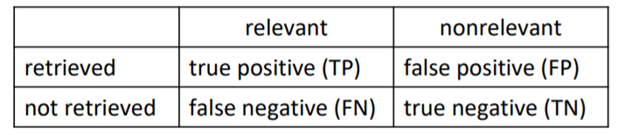
\includegraphics[scale=0.9]{p1.png}
    \caption{Confusion Matrix}
    \label{fig:my_label}
\end{figure}
\begin{itemize}
    \item Precision : fraction of retrieved documents that are relevant. Recall: fraction of relevant documents that were retrieved.
    
    \item Precision prefers systems that retrieve less number of highly relevant documents, Recall prefers high number of retrieved documents. 
    
    \item Precision decreases as the number of retrieved documents increases (unless in perfect ranking), while recall keeps increasing 
    
    \item The F-score is a combination of the precision and recall:
    \begin{align}
        P &= \frac{TP}{TP+TN} \\
        R &= \frac{TP}{TP+FN} \\
        F &= \frac{1}{\frac{\alpha}{P} + \frac{1-\alpha}{R}}
    \end{align}
    
    \item The HM is used as it is a smooth minimum, and it punishes bad performance on either the P or the R. It is known that $HM \le GM \le AM$
    
    \item AM for a naive engine that simply returns everything as result is 0.5  which is too high. 
\end{itemize}

\subsection{Ranked Evaluation}
\begin{itemize}
    \item Equation (3) can also be written as
    \begin{align}
        F &= \frac{1}{\frac{\alpha}{P} + \frac{1-\alpha}{R}} = \frac{(\beta+1)PR}{\beta P + R} \\
        \beta &= \frac{1-\alpha}{\alpha}
    \end{align}
    
    \item $\beta < 1$ emphasizes precision, $\beta > 1$ emphasizes recall.
    
    \item On one query, different systems tend to perform the same. On different queries, there is large variance in performance of a single system 
    
    \item COmputing P and R for top 1, 2, 3, 4, and so on documents leads to a P-R curve (P on vertical, R on horizontal). A P-R curve is a sawtooth:
    \begin{itemize}
        \item Next document considered is irrelevant, hence recall constant but precision reduces (vertical decrease)
        
        \item Next document considered is relevant, hence recall and precision increase, a rightward upward movement. 
    \end{itemize}
    
    \item Interpolate the points by taking maximum of all future points
    
    \item The \textbf{Mean Average Precision} (MAP) is a summary measure derived from the graph. 
    
    \item For single information need, average precision is the average of the precision value obtained for the set of top K documents existing after each relevant document is retrieved
    
    \item MAP is the average of average precisions over all the queries considered. 
    
    \item For a single query, average precision approximates the area under the precision recall curve
    
    \item Set of information needs should be diverse for MAP to be an effective measure across systems
\end{itemize}

\end{document}